\documentclass{article}

\usepackage{graphicx}
\usepackage{tikz}
\usepackage{tikzsymbols}
\usetikzlibrary{calc,patterns,shapes.geometric}
\pagestyle{empty}
\usepackage[margin=0pt]{geometry}
\geometry{papersize={14in,12in}}

\def\centerarc[#1](#2)(#3:#4:#5){\draw[#1] ($(#2)+({#5*cos(#3)},{#5*sin(#3)})$) arc (#3:#4:#5);}

\begin{document}
	\begin{figure}
		\centering
		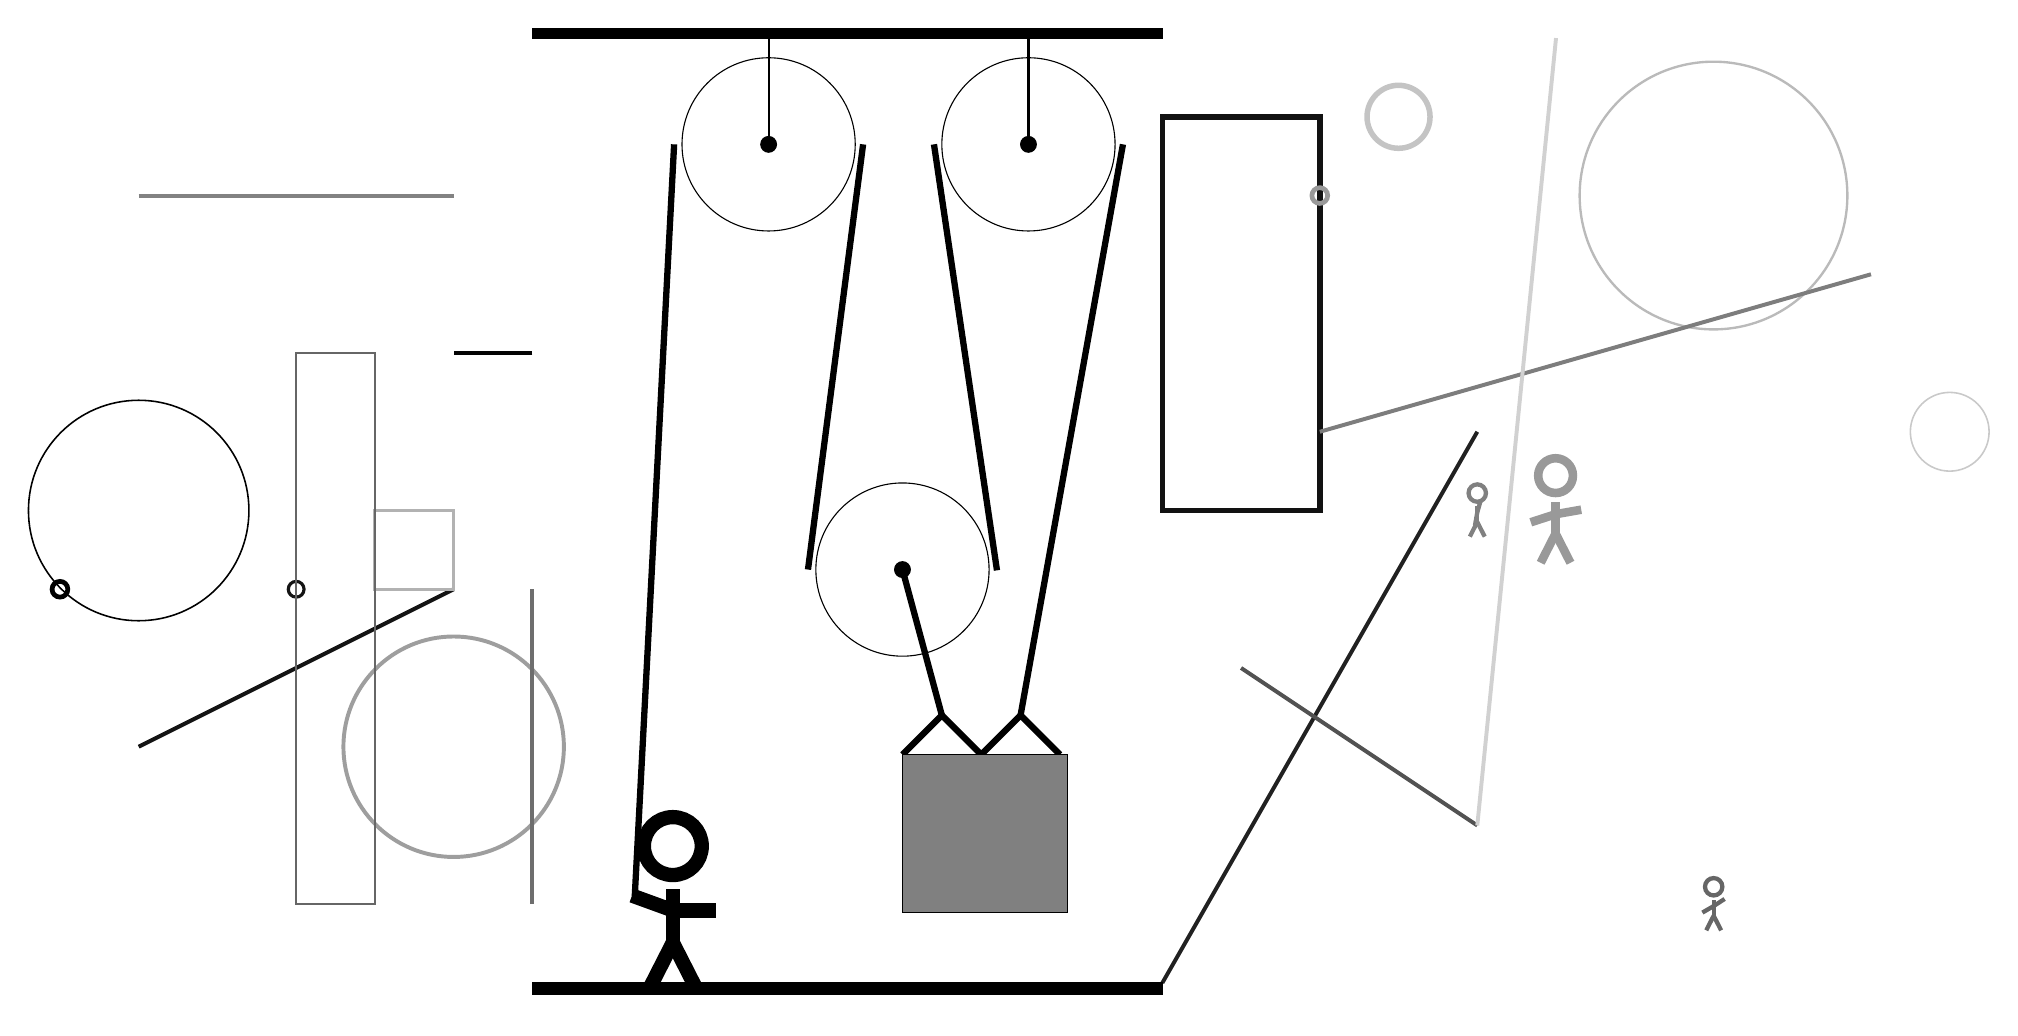
\begin{tikzpicture}
			%%%%% START %%%%%
			
			\draw[fill=black] (-2, 9) rectangle (6, 9.125);
			
			\draw (1, 7.65) circle (1.1);
			\draw[fill=black] (1, 7.65) circle (0.1);
			\draw[thick] (1, 7.65) -- (1, 9);
			
			\draw (4.3, 7.65) circle (1.1);
			\draw[fill=black] (4.3, 7.65) circle (0.1);
			\draw[thick] (4.3, 7.65) -- (4.3, 9);
			
			\draw (2.7, 2.25) circle (1.1);
			\draw[fill=black] (2.7, 2.25) circle (0.1);
			
			\draw[line width=0.8mm]  (2.7, -0.1) -- (3.2, 0.4) -- (3.7, -0.1) -- (4.2, 0.4) -- (4.7, -0.1);
			\draw[fill=black!50] (2.7, -0.1) rectangle (4.8, -2.1);
			
			\draw[line width=0.5mm, color=black!87](10, 4) -- (6, -3);
			
			\draw [line width=0.2mm, color=black!100](-7, 3) circle (1.4);
			\draw[line width=0.7mm, color=black!93] (8, 8) rectangle (6, 3);
			\draw [line width=0.4mm, color=black!92](-5, 2) circle (0.1);
			\draw[line width=0.5mm, color=black!92](-7, 0) -- (-3, 2);
			
			\draw [line width=0.7mm, color=black!23](9, 8) circle (0.4);
			\draw [line width=0.6mm, color=black!100](-8, 2) circle (0.1);
			\draw [line width=0.6mm, color=black!40](8, 7) circle (0.1);
			\node[line width=0.7mm, color=black!50] at (10, 3) {\Strichmaxerl[3][80][74]};
			\draw[line width=0.5mm, color=black!49](-7, 7) -- (-3, 7);
			
			\draw [line width=0.3mm, color=black!27](13, 7) circle (1.7);
			\draw [line width=0.5mm, color=black!38](-3, 0) circle (1.4);
			\draw[line width=0.5mm, color=black!99](-2, 5) -- (-3, 5);
			
			\draw [line width=0.2mm, color=black!21](16, 4) circle (0.5);
			\node[line width=0.5mm, color=black!40] at (11, 3) {\Strichmaxerl[6][18][10]};
			\draw[line width=0.5mm, color=black!26] (-3, 6) rectangle (-3, 6);
			
			\draw[line width=0.5mm, color=black!51](8, 4) -- (15, 6);
			\draw[line width=0.5mm, color=black!57](-2, -2) -- (-2, 2);
			\draw[line width=0.5mm, color=black!68](10, -1) -- (7, 1);
			\draw[line width=0.4mm, color=black!30] (-3, 3) rectangle (-4, 2);
			\node[line width=0.6mm, color=black!60] at (13, -2) {\Strichmaxerl[3][30][33]};
			
			\draw[line width=0.2mm, color=black!60] (-4, -2) rectangle (-5, 5);
			\draw[line width=0.5mm, color=black!18](10, -1) -- (11, 9);
			
			\draw[line width=0.8mm](-0.7, -1.9) -- (-0.2, 7.65);
			\centerarc[line width=0.8mm](1, 7.65)(0:180:1.2000000000000002);
			\draw[line width=0.8mm](2.2, 7.65) -- (1.5, 2.25);
			\centerarc[line width=0.8mm](2.7, 2.25)(180:370:1.2000000000000002);
			\draw[line width=0.8mm] (3.9, 2.24) -- (3.1, 7.65);
			\centerarc[line width=0.8mm](4.3, 7.65)(0:180:1.2000000000000002);
			\draw[line width=0.8mm](4.2, 0.4) -- (5.5, 7.65);
			\draw[line width=0.8mm] (3.2, 0.4) -- (2.7, 2.25);
			
			\node at (-0.2, -2) {\Strichmaxerl[10][-20][0]};
			
			\draw[fill=black] (-2, -3) rectangle (6, -3.15);
			
			%%%%% END %%%%%
		\end{tikzpicture}
	\end{figure}	
\end{document}